\documentclass[a4paper]{article}
\usepackage[italian]{babel}
\usepackage[style=ieee,backend=biber]{biblatex} \addbibresource{bibliography.bib}
\usepackage{csquotes}
\usepackage{hyperref}
\usepackage{algorithm}
\usepackage{algpseudocode}
\usepackage[table]{xcolor}
\usepackage{minted}
\usepackage{amsmath}
\usepackage{listings}
\usepackage{xcolor}
\usepackage{graphicx}
\usepackage{hyperref}
\DeclareMathOperator{\lcm}{lcm}

\lstset{
    language=C++,
    basicstyle=\ttfamily\small,
    keywordstyle=\color{blue},
    commentstyle=\color{gray},
    stringstyle=\color{red},
    numbers=left,
    numberstyle=\tiny\color{gray},
    stepnumber=1,
    numbersep=10pt,
    tabsize=2,
    showspaces=false,
    showstringspaces=false,
    breaklines=true,
    frame=single,
    backgroundcolor=\color{lightgray},
    captionpos=b
}

\title{Report PHPC}
\author{Pierluigi Supino \and Rodolfo Diana \and Salvatore Di Gennaro}

\begin{document}

\maketitle
\tableofcontents

\section{Introduzione}

Sviluppare un’applicazione per il prodotto tra matrici su cluster multi-nodo e multi-GPU per nodo (MPI + CUDA, attraverso SLURM). All’interno di questa applicazione devono essere possibili entrambe le seguenti:
\begin{enumerate}
    \item utilizzare kernel originali per i calcoli sulla GPU;
    \item utilizzare funzioni della libreria cuBLAS in alternativa a quelle originali.
\end{enumerate}

\section{Implementazione}
In un ambiente multi-nodo e multi-GPU, il prodotto tra matrici può essere articolato in due livelli distinti ma interconnessi.

A un livello più alto è necessario decomporre il problema a livello globale, ovvero suddividere le matrici da moltiplicare in blocchi che possano essere assegnati in modo efficiente ai diversi nodi del cluster, tenendo conto del bilanciamento del carico, della minimizzazione della comunicazione tra nodi e dell'architettura del sistema.

A un livello più basso, invece, entra in gioco l’effettiva esecuzione del prodotto tra i blocchi locali di matrici all’interno di ciascun nodo, sfruttando le GPU a disposizione. Si potrebbe ulteriormente suddividere questo livello in partizionamento delle matrice tra le diverse GPU ed esecuzione dei calcoli.

\subsection{Processi}
Il prodotto tra matrici viene eseguito a livello di processi tramite SUMMA (Scalable Universal Matrix Multiplication Algorithm)\cite{SUMMA}.
Si dispongano i diversi processi in una griglia logica bidimensionale $r \times c$ e sia $l=\lcm(r, c)$. È possibile suddividere le matrici nel seguente modo:
$$
    \mathbf{A}=
    \begin{pmatrix}
        \mathbf{A}_{00}     & \cdots & \mathbf{A}_{0(l-1)}     \\
        \vdots              & \ddots & \vdots                  \\
        \mathbf{A}_{(r-1)0} & \cdots & \mathbf{A}_{(r-1)(l-1)}
    \end{pmatrix}
$$

$$
    \mathbf{B}=
    \begin{pmatrix}
        \mathbf{B}_{00}     & \cdots & \mathbf{B}_{0(c-1)}     \\
        \vdots              & \ddots & \vdots                  \\
        \mathbf{B}_{(l-1)0} & \cdots & \mathbf{B}_{(l-1)(c-1)}
    \end{pmatrix}
$$

$$
    \mathbf{C}=
    \begin{pmatrix}
        \sum_{k=0}^{l-1}\mathbf{A}_{0k}\mathbf{B}_{k0}     & \cdots & \sum_{k=0}^{l-1}\mathbf{A}_{0k}\mathbf{B}_{k(c-1)}     \\
        \vdots                                             & \ddots & \vdots                                                 \\
        \sum_{k=0}^{l-1}\mathbf{A}_{(r-1)k}\mathbf{B}_{k0} & \cdots & \sum_{k=0}^{l-1}\mathbf{A}_{(r-1)k}\mathbf{B}_{k(c-1)}
    \end{pmatrix}
$$

Ad ogni processo $P_{ij}$ vengono assegnati i blocchi $\mathbf{A}_{is}$ per cui $\bmod(s,l)=j$, e i blocchi $\mathbf{B}_{tj}$ per cui $\bmod(t,l)=i$. L'algoritmo si svolge in più passaggi nei quali i processi collaborano per combinare blocchi specifici. Ad ogni passo $k$, il processo che possiede il blocco $\mathbf{A}_{ik}$ lo invia alla propria riga e, analogamente, il possessore del blocco $\mathbf{B}_{kj}$ alla propria colonna.
Una volta ricevuti i blocchi necessari, ogni processo può calcolare una parte del prodotto parziale della matrice $\mathbf{C}$, sommando il risultato a quello già accumulato. Ripetendo questa operazione, alla fine ogni processo avrà calcolato il suo blocco completo di $\mathbf{C}$.

\begin{algorithm}[h]
    \caption{SUMMA for process $P_{ij}$}
    \begin{algorithmic}
        \State $\mathbf{C}_{ij} \gets 0$
        \State $l \gets \lcm(r,c)$
        \For{$k \gets 0$ \textbf{to} $l - 1$}
        \State $s \gets \bmod(k, r)$
        \State $t \gets \bmod(k, c)$
        \State process $P_{it}$ broadcasts $\mathbf{A}_{ik}$ to row
        \State process $P_{sj}$ broadcasts $\mathbf{B}_{kj}$ to column
        \State $\mathbf{C}_{ij} \gets \mathbf{C}_{ij} + \mathbf{A}_{ik}\mathbf{B}_{kj}$
        \EndFor
    \end{algorithmic}
\end{algorithm}

L'ultimo passaggio consiste nel ricomporre le diverse sottomatrici dai vari processi, risolvibile con diversi approcci a seconda di come sia necessario il risultato.

\medskip Nell'implementazione attuale, per semplicità, le matrici $\mathbf{A}, \mathbf{B}$ in input devono essere dei quadrati $n \times n$ dove $n = q \cdot \lcm(r,c)$ per qualche $q \ge 1$, allocate come array contigui \textit{row-major} e contenere già al loro interno (almeno) i dati dei blocchi assegnati al processo chiamante.

L'invio dei blocchi avviene tramite un'operazione di broadcast dello standard di comunicazione \textit{Message Passing Interface} (MPI)\footnote{\url{https://docs.open-mpi.org/en/v5.0.x/man-openmpi/man3/MPI_Bcast.3.html}}.
Siccome bisogna inviare porzioni di una matrice più grande, è stato necessario creare dei tipi derivati appositi per tenere in considerazione gli spazi di memoria che intercorrono tra una riga e l'altra dei blocchi da inviare\footnote{\url{https://docs.open-mpi.org/en/v5.0.x/man-openmpi/man3/MPI_Type_vector.3.html}}.

$$
    \begin{pmatrix}
        \color{red} x_{00} & \color{red} x_{01} & x_{02} & \cdots & x_{0n} \\
        \color{red} x_{10} & \color{red} x_{11} & x_{12} & \cdots & x_{1n} \\
        x_{20}             & x_{21}             & x_{22} & \cdots & x_{2n} \\
                           &                    & \cdots &        &        \\
    \end{pmatrix}
$$

$$
    \begin{pmatrix}
        \color{red} x_{00} & \color{red} x_{01} & x_{02} & \cdots & x_{0n} & \color{red} x_{10} & \color{red} x_{11} & x_{12} & \cdots
    \end{pmatrix}
$$

Per quanto riguarda la ricomposizione di $\mathbf{C}$, è stato deciso che solo il processo 0 debba avere la matrice finale completa.
Non è stata implementata una particolare gestione degli errori per evitare overhead nelle misurazioni dei tempi.

\subsection{GPU}
\subsubsection{Multi-GPU}
Per sfruttare al massimo le risorse disponibili, è stato necessario sviluppare un sistema che permettesse la suddivisione del lavoro su più GPU presenti nella macchina.

L'obiettivo consiste nel sovrapporre quanto più possibile il lavoro svolto dalle diverse GPU ed evitare conflitti di memoria che dovrebbero essere serializzati, in particolare la scrittura sulla matrice $\mathbf{C}$. Un'idea naturale è partizionare quest'ultima in modo che ogni device possa eseguire le operazioni in uno spazio separato dagli altri.
Una suddivisione semplice ma funzionale per qualsiasi numero di GPU è quella per colonne: ogni GPU effettua quindi il prodotto tra la matrice $\mathbf{A}$ e la ``colonna'' assegnata della matrice $\mathbf{B}$.

$$
    \mathbf{B}=
    \begin{pmatrix}
        \mathbf{B}_{0} & \cdots & \mathbf{B}_{n - 1} \\
    \end{pmatrix}\\
$$
$$
    \mathbf{C}=
    \begin{pmatrix}
        \mathbf{A}\mathbf{B}_0 & \cdots & \mathbf{A}\mathbf{B}_{n-1} \\
    \end{pmatrix}
$$

Questo meccanismo implica, ovviamente, che l'host debba essere in grado di avviare l'esecuzione su più GPU senza dover attendere prima il completamento di una di esse.
Un metodo sicuramente valido è creare diversi thread a livello di processo, ognuno dei quali gestisca un determinato device.
Tuttavia, CUDA offre anche varianti asincrone delle diverse funzioni e la possibilità di gestirle tramite \textit{stream}, ovvero code di operazioni da eseguire in sequenza.

% TODO: aggiungere pseudocodice
% \begin{algorithm}[h]
%     \caption{MultiGPU}
%     \begin{algorithmic}
%         \For{$i \gets 0$ \textbf{to} $n - 1$}
%         \State create stream $s_i$
%         \State allocate memory async on device
%         \State $C_i \gets cudaMemcpy()$
%         \State $C_{ij} \gets C_{ij} + AB$
%         \EndFor
%         \For{$i \gets 0$ \textbf{to} $n - 1$}
%         \State wait stream $i$
%         \State destroy stream $i$
%         \EndFor
%     \end{algorithmic}
% \end{algorithm}

\subsubsection{Kernel}

La moltiplicazione tra una matrice M $(I\times{J})$ e una matrice N $(J\times{K})$ produce una matrice P $(I\times{K})$. Ognuno degli elementi della matrice $P$ è il prodotto scalare tra una riga di $M$ e una colonna di $N$. Riferendoci agli elementi di $P$ con $P_{\text{row}, \text{col}}$ avremo:

\[
    P_{\text{row}, \text{col}} = \sum_{k=0}^{\text{Width}-1} M_{\text{row}, k} \cdot N_{k, \text{col}}
\]

Ovvero per calcolare ad esempio l'elemento $P_{1, 5}$:

\[
    P_{1,5} = M_{1,0} \cdot N_{0,5} + M_{1,1} \cdot N_{1,5} + M_{1,2} \cdot N_{2,5} + \ldots + M_{1,\text{width}-1} \cdot N_{\text{width}-1,5}
\]

Per implementare la moltiplicazione tra matrici usando CUDA, possiamo mappare i thread nelle griglia agli elementi della matrice di output $P$. In questo modo, ogni thread sarà responsabile del calcolo di un elemento di $P$. Gli indici di colonna per gli elementi di $P$ sarano:

\[
    \begin{aligned}
        \text{row} & = \text{blockIdx.y} \times \text{blockDim.y} + \text{threadIdx.y} \\
        \text{col} & = \text{blockIdx.x} \times \text{blockDim.x} + \text{threadIdx.x}
    \end{aligned}
\]

Con questo mapping uno a uno il nostro kernel sarà:

\begin{lstlisting}[caption={Kernel CUDA con memoria globale}, label={lst:1}]
__global__ void MatrixMulKernel(float* M, float* N,
                                float* P, int Width) {
    int row = blockIdx.y*blockDim.y+threadIdx.y;
    int col = blockIdx.x*blockDim.x+threadIdx.x;
    if ((row < Width) && (col < Width)) {
        float Pvalue = 0;
        for (int k = 0; k < Width; ++k) {
            Pvalue += M[row*Width+k]*N[k*Width+col];
        }
        P[row*Width+col] = Pvalue;
    }
}
\end{lstlisting}

\newpage

La Figura~\ref{fig:1}, mostra come viene suddivisa la matrice $P$ ($4\times{4}$) in una griglia di blocchi $2\times{2}$ con blocchi $2\times{2}$. Mentre la Figura~\ref{fig:2} ne mostra una parte dell'esecuzione.

\begin{figure}[H]
    \centering
    \begin{minipage}[b]{0.45\textwidth}
        \centering
        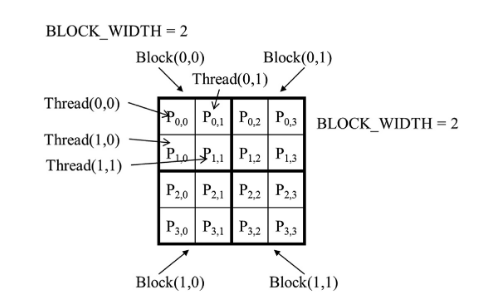
\includegraphics[width=\textwidth]{imgs/matrix_division.png}
        \caption{Divisione della matrice in una griglia di blocchi}
        \label{fig:1}
    \end{minipage}
    \hspace{0.05\textwidth}
    \begin{minipage}[b]{0.45\textwidth}
        \centering
        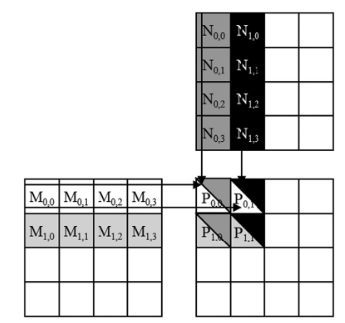
\includegraphics[width=\textwidth]{imgs/execution1.png}
        \caption{Esecuzione del kernel}
        \label{fig:2}
    \end{minipage}
\end{figure}

Questo è un approccio basilare con ampi margini di miglioramento, infatti in un contesto CUDA è fondamentale ragionare tenendo in considerazione le differenti prestazioni delle differenti memorie: la memoria globale è grande ma lenta di controparte la memoria condivisa è piccola ma veloce. Una strategia decisamente migliore rispetto a quella presentata in precedenza è quella di partizionare i dati in sottoinsiemi chiamati \textit{tiles} in modo tale che ognuna di essa entri nella memoria condivisa con un importante vincolo, la computazione del kernel sulla singola tile può essere fatta indipendentemente dalle altre. Tornando all' esempio precedente mostriamo gli accessi alla memoria globale generati dal'esempio in Figura~\ref{fig:2}:

\begin{figure}[H]
    \centering
    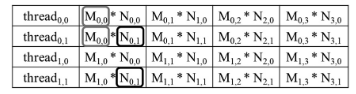
\includegraphics[width=0.6\textwidth]{imgs/memory_access.png}
    \caption{Accessi alla memoria globale}
    \label{fig:3}
\end{figure}

Nella Figura~\ref{fig:3} possiamo notare come gli stessi elementi vengano letti dalla lenta memoria globale in diversi step dell'esecuzione. In generale data la dimensione dei blocchi $width\times{width}$ ogni elemento delle matrici $M$ ed $N$ è letto dalla memoria globale $width$ volte. L'idea è quindi quella di far collaborare i threads per caricare in memoria condivisa anticipatamente tutti i dati per poi procedere allo sviluppo dei calcoli cosi facendo stiamo riducendo di $\frac{1}{width}$ gli accessi alla memoria. La Figura~\ref{fig:1} mostra gli accessi alla memoria per questo approccio.

\begin{figure}[H]
    \centering
    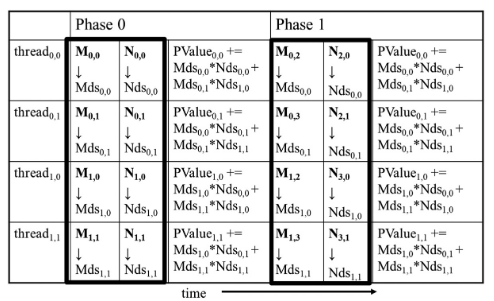
\includegraphics[width=0.6\textwidth]{imgs/memory_access1.png}
    \caption{Accessi alla memoria globale e caricamento in memoria condivisa}
    \label{fig:4}
\end{figure}

Il Listing~\ref{lst:2} mostra il kernel con l'approccio tiling e memoria condivisa.

\begin{lstlisting}[caption={Kernel CUDA con tiling e memoria condivisa}, label={lst:2}]
#define TILE_WIDTH 16
__global__ void matrixMulKernel(float* M, float* N, float* P, int Width) {
    __shared__ float Mds[TILE_WIDTH][TILE_WIDTH];
    __shared__ float Nds[TILE_WIDTH][TILE_WIDTH];

    int bx = blockIdx.x; int by = blockIdx.y;
    int tx = threadIdx.x; int ty = threadIdx.y;

    int Row = by * TILE_WIDTH + ty;
    int Col = bx * TILE_WIDTH + tx;

    float Pvalue = 0;
    for (int ph = 0; ph < Width/TILE_WIDTH; ++ph) {
        Mds[ty][tx] = M[Row*Width + ph*TILE_WIDTH + tx];
        Nds[ty][tx] = N[(ph*TILE_WIDTH + ty)*Width + Col];
        __syncthreads();

        for (int k = 0; k < TILE_WIDTH; ++k)
            Pvalue += Mds[ty][k] * Nds[k][tx];
        __syncthreads();
    }
    P[Row*Width + Col] = Pvalue;
}
\end{lstlisting}

\newpage

Il Listing~\ref{lst:2} nonostante ottimizzi l'uso delle memorie non funzionerebbe con matrici la cui $widht$ non sia un multiplo di $TILE\_WIDHT$ nel Listing~\ref{lst:3} è mostrata la soluzione approssimando per eccesso la divisione per $TILE\_WIDTH$ e riempendo con degli $0$ le parti di tile che non vanno effettivamente utilizzate

\begin{lstlisting}[caption={Kernel CUDA con gestione dei bordi e tiling}, label={lst:3}]
float Pvalue = 0;
for (int ph = 0; ph < ceil(Width/(float)TILE_WIDTH); ++ph) {

    if ((Row < Width) && (ph*TILE_WIDTH+tx) < Width)
        Mds[ty][tx] = M[Row*Width + ph*TILE_WIDTH + tx];
    else
        Mds[ty][tx] = 0.0f;

    if ((ph*TILE_WIDTH+ty < Width) && (Col < Width))
        Nds[ty][tx] = N[(ph*TILE_WIDTH + ty)*Width + Col];
    else
        Nds[ty][tx] = 0.0f;

    __syncthreads();

    for (int k = 0; k < TILE_WIDTH; ++k)
        Pvalue += Mds[ty][k] * Nds[k][tx];

    __syncthreads();
}

if (Row < Width && Col < Width)
    P[Row*Width + Col] = Pvalue;
\end{lstlisting}

Il nostro scopo era quello di testare l'andamento delle prestazioni al variare del numero di thread e processi questo per quanto riguarda il kernel ne comporta l'adattamento in modo tale che un qualsiasi numero di thread (anche solo 1) possa effettuare in autonomia l'intero calcolo. Il Listing~\ref{lst:4} mostra questo adattamento con un grid-stride-loop. Si noti anche la definizione dinamica della memoria condivisa, in particolare viene usato 1 singolo array \textit{shared\_mem} la cui dimensione sarà uguale a $2\times{TILE\_WIDTH}\times{sizeof(double)}$ ovvero stiamo allocando lo spazio in memoria condivisa per salvare in modo contiguo nello stesso array le $2$ tile correnti da moltiplicare. Questo valore per assicurare le massime prestazioni dovrà essere $\leq cudaDevAttrMaxSharedMemoryPerBlock$ ovvero il limite hardware imposto dall'architettura della GPU che si sta usando.

\begin{lstlisting}[caption={Kernel CUDA generalizzato con tiling dinamico}, label={lst:4}]
__global__ void matrixMulKernel(double *A, double *B, double *C, int M, int N, int K) {
    extern __shared__ double shared_mem[];

    int tile_width = blockDim.x;

    double *s_A = (double *)shared_mem;
    double *s_B = (double *)shared_mem + tile_width * tile_width;

    int tx = threadIdx.x;
    int ty = threadIdx.y;

    int num_tiles_N = ceil((double)N / tile_width);
    int num_tiles_M = ceil((double)M / tile_width);
    int total_tiles = num_tiles_M * num_tiles_N;

    int block_id_1d = blockIdx.y * gridDim.x + blockIdx.x;
    int total_blocks = gridDim.x * gridDim.y;

    for (int tile_id = block_id_1d; tile_id < total_tiles; tile_id += total_blocks) {
        int by_tile = tile_id / num_tiles_N;
        int bx_tile = tile_id % num_tiles_N;

        int global_row = by_tile * tile_width + ty;
        int global_col = bx_tile * tile_width + tx;

        double c_value = 0.0;
        int phases = (K + tile_width - 1) / tile_width;

        for (int phase = 0; phase < phases; ++phase) {
            if ((global_row < M) && (phase * tile_width + tx < K))
                s_A[ty * tile_width + tx] = A[global_row * K + phase * tile_width + tx];
            else
                s_A[ty * tile_width + tx] = 0.0;

            if ((phase * tile_width + ty < K) && (global_col < N))
                s_B[ty * tile_width + tx] = B[(phase * tile_width + ty) * N + global_col];
            else
                s_B[ty * tile_width + tx] = 0.0;

            __syncthreads();

            for (int k = 0; k < tile_width; ++k)
                c_value += s_A[ty * tile_width + k] * s_B[k * tile_width + tx];

            __syncthreads();
        }

        if ((global_row < M) && (global_col < N))
            C[global_row * N + global_col] = c_value;
    }
}
\end{lstlisting}

\subsubsection{cuBLAS}
In alternativa a scrivere le proprie funzioni per il calcolo tra matrici, è disponibile la libreria cuBLAS sviluppata da NVIDIA che fornisce una versione ottimizzata per GPU delle routine BLAS (Basic Linear Algebra Subprograms), una serie standard di operazioni fondamentali in algebra lineare\footnote{\url{https://netlib.org/blas/}}. Sono inoltre disponibili diverse estensioni, tra cui cuBLASXt progettata per sfruttare più GPU contemporaneamente. Non sono necessari preparativi particolari, dato che si occupa autonomamente di allocare la memoria tra le GPU designate, distribuire il carico di lavoro tra di loro e infine recuperare i risultati sull'host\footnote{\url{https://docs.nvidia.com/cuda/cublas/index.html\#using-the-cublasxt-api}}.

Una nota tecnica riguarda la discrepanza tra l'ordine in memoria delle matrici: cuBLAS, per rimanere conforme alle specifiche Fortran di BLAS, si aspetta che i valori siano disposti per \textit{column-major} mentre lo standard nel C è \textit{row-major}. Fortunatamente, è possibile evitare operazioni di memoria aggiuntive il fatto che i due metodi sono le rispettive trasposte e calcolare
$$
    \mathbf{C}^T=(\mathbf{B}\mathbf{A})^T
$$
Il risultato sarà quindi salvato in una matrice column-major e che quindi corrisponderà al risultato cercato leggendolo in row-major.

\section{Analisi}

\subsection{Ambiente di test}

TODO Pier: IBISCO

\subsection{Configurazione dei test}

TODO Pier: SCRIPT E CSV (per configurazione test)

\subsection{Analisi delle misurazioni}

\subsection{NVIDIA Nsight Compute}

\section{Esplorazione di NNCL}

\subsection{Introduzione}

\subsection{Possibili implementazioni}

\printbibliography

\end{document}